
\documentclass[11pt,conference,compsoc]{IEEEtran}
\usepackage{graphicx}
\usepackage{listings}
\usepackage{algpseudocode}
\usepackage{booktabs}

\usepackage{tabularx}
\usepackage{hyperref}
\usepackage{amsmath}
\usepackage{microtype}
\usepackage{parskip}
\usepackage{titlesec}
\usepackage{enumitem}
\usepackage{xcolor}
\usepackage{url}
\ifCLASSOPTIONcompsoc
  % IEEE Computer Society needs nocompress option
  % requires cite.sty v4.0 or later (November 2003)
  \usepackage[nocompress]{cite}
\else
  % normal IEEE
  \usepackage{cite}
\fi

\usepackage{dirtytalk}


% *** GRAPHICS RELATED PACKAGES ***
%
\ifCLASSINFOpdf
  % \usepackage[pdftex]{graphicx}
  % declare the path(s) where your graphic files are
  % \graphicspath{{../pdf/}{../jpeg/}}
  % and their extensions so you won't have to specify these with
  % every instance of \includegraphics
  % \DeclareGraphicsExtensions{.pdf,.jpeg,.png}
\else

\fi



% correct bad hyphenation here
\hyphenation{op-tical net-works semi-conduc-tor}


\begin{document}
%
% paper title
% Titles are generally capitalized except for words such as a, an, and, as,
% at, but, by, for, in, nor, of, on, or, the, to and up, which are usually
% not capitalized unless they are the first or last word of the title.
% Linebreaks \\ can be used within to get better formatting as desired.
% Do not put math or special symbols in the title.
\title{Examining Language Model Reasoning with Minesweeper Puzzle Variants}


% author names and affiliations
% use a multiple column layout for up to three different
% affiliations
\author{
\IEEEauthorblockN{Evan Economou}
\IEEEauthorblockA{\footnotesize Colorado School of Mines\\
$\left<{\rm eeconomou@mines.edu}\right>$}\\
}





% use for special paper notices
%\IEEEspecialpapernotice{(Invited Paper)}




% make the title area
\maketitle

% As a general rule, do not put math, special symbols or citations
% in the abstract
\begin{abstract}
As language models evolve so rapidly, it is important to be able to benchmark and document the growth and change in their capabilities. They have demonstrated remarkable emergent reasoning capabilities, repeatedly demonstrating the ability to effectively synthesize new information and tackle problems.
In this paper, I utilize the puzzle game Minesweeper alongside additional rulesets (``variants") to try to create a rigid structure in which to examine these capabilities, taking advantage of Minesweeper's deterministic problem space while using variants to enforce a need for creativity in puzzle solving.
Contrary to the initial hypothesis that constraints that affected the board at a global scale would be the most difficult, the models struggled most heavily with variants that modified the semantic meaning of clues away from traditional Minesweeper rules.
\end{abstract}


\IEEEpeerreviewmaketitle

% ***********************************************************************
% * Alex's Code: https://github.com/chenota/des-analysis
% * Using this link: https://link.springer.com/article/10.1007/BF00630563
% ***********************************************************************

\section{Introduction}
% (including the background, motivation, and goal)

As large language models (LLMs) have grown in capability, the research community has increasingly turned to controlled, rule-governed environments to probe the boundary between genuine reasoning and sophisticated pattern-matching on training data. Often this is in pursuit of the interesting and ongoing question of to what extent language models can reason about concepts and processes that weren't explicitly included in training~\cite{brown2020gpt3,wei2022emergent}. This concern is especially relevant for many existing benchmarks, which can inadvertently reward recall from training data rather than creativity~\cite{li2024minesweeper}.

One productive avenue of exploration has been to evaluate LLMs inside discrete game environments, where the rules are unambiguous, success is verifiable, and the action space is well-defined. The formal rule structures of games allow researchers to construct novel configurations that are structurally similar to, but semantically distinct from, anything plausibly in an LLM's training data~\cite{liu2023agentbench,hu2025gamearena,seely2025sudoku}. Puzzle-based evaluations have extended this line of work to single-agent settings where logical deduction is the primary skill under examination. Xu et al.~\cite{xu2024puzzlesurvey} survey a range of such puzzle-based benchmarks and find that LLMs consistently struggle to maintain multi-step deductive chains, even when individual reasoning steps are within reach. A closely related study by Seely et al.~\cite{seely2025sudoku} used unconventional Sudoku variants as a test bed, selecting puzzles with novel interacting constraints specifically to defeat memorization; state-of-the-art models solved fewer than 15\% of puzzles unaided.

Minesweeper is a particularly appealing evaluation domain because it can be formalized as a well defined constraint satisfaction problem~\cite{studholme2001minesweeper}, its rules are compact and unambiguous, and the gap between understanding a rule and correctly applying it across an evolving board state is large enough to expose meaningful differences in reasoning quality. Prior work has taken this gamification of benchmarks and examined Minesweeper specifically. Li et al.~\cite{li2024minesweeper} conducted experiments with GPT-3.5 and GPT-4, finding that the models were able to understand individual board states and identify which cells a numeric clue constrained, but struggled to chain those inferences into a coherent multi-step solving strategy. That study also identified a tendency for LLMs to produce sequences of actions that are locally plausible but globally incoherent, behaving more like a heuristic search than a true deduction.

This paper builds on this prior work by asking a different question: rather than varying board difficulty or size, what happens to the model's ability to reason when the rules themselves are modified? I utilize twelve Minesweeper variants drawn from the game \textit{14~Minesweeper Variants}~\cite{artlessgames2022minesweeper} and organized into two categories: structural variants, which impose additional constraints on where mines may appear but leave clue semantics intact, and clue-modifier variants, which change what the displayed numeric values mean. This design attempts to isolates two main distinct competencies. The first is the ability to incorporate additional global constraints while still applying familiar deductive patterns, a capacity for additive reasoning under rule augmentation. The second is the ability to fully reinterpret a learned symbol system when its semantics change, the capacity for semantic recalibration that goes beyond adding information to an existing framework.

My findings reveal a stark asymmetry between these two types of reasoning. \texttt{claude-haiku-4-5}, evaluated via the Anthropic API with extended thinking enabled, achieved win rates up to $60\%-86\%$ across most structural variants but $0\%$ on all three clue-modifier variants. Losses in the clue-modifier condition were not gradual, and in the Liar and Partition variants the model hit a mine on nearly every first move, performing worse than a random agent.
Examination of the extended thinking traces shows that the model could reproduce the variant rule when prompted but then reasoned from standard Minesweeper semantics anyway, suggesting that surface-level rule comprehension does not propagate into the underlying inference procedure when the variant directly conflicts with a well-learned pattern.

This paper presents two primary contributions:
\begin{enumerate}
    \item A puzzle-based evaluation framework using twelve Minesweeper rule variants
          that cleanly separates structural rule augmentation from semantic rule
          substitution as sources of difficulty for LLMs.
    \item Evidence towards the idea that LLMs are more robust to additive
          structural constraints than to modifications of familiar symbol semantics,
          with implications for how reasoning benchmarks should be designed.
\end{enumerate}


\section{Background}
% (e.g., survey, testbed, system design/implementation, experiments, etc.) with justification (i.e., why they are reasonable and meaningful)

\subsection{Minesweeper}
Minesweeper is a classic game of logical deduction where the player's goal is to reveal all safe cells on a board without revealing any mines. Each cell on the board can exist in a few different states:
\begin{itemize}
    \item Hidden (``\#"): These cells haven't been revealed yet, and can still be transformed into any of the following states
    \item Numbered (``1" to "8"): These cells contain the number of mines in the 8 adjacent cells
    \item Empty (``."): These cells have no mines adjacent to them, but have been revealed
    \item Flagged (``F"): Cells that have been marked as a mine

\end{itemize}
Using these rules, standard minesweeper can be formulated as a constraint satisfaction problem\cite{studholme2001minesweeper}. Each revealed numeric cell creates a linear constraint over the status of implicit binary mine or non-mine variable for the unrevealed neighbors. This gives the game a strong basis to be used as a reasoning benchmark.
\subsection{Variants}
The board variants in this study are drawn from the game \textit{14 Minesweeper
Variants} ~\cite{artlessgames2022minesweeper} and organized into two broad categories.

\textbf{Structural (placement) constraints}, as seen in Table \ref{tab:structural} modify where mines may appear but leave
the clue values unchanged. The revealed number on a cell still counts mines in the
standard eight-cell neighborhood.
\begin{table}[htp]
\centering
\small
\begin{tabularx}{\columnwidth}{@{}llX@{}}
\toprule
Code & Name & Rule \\
\midrule
Q & Quad      & Every $2{\times}2$ block contains at least one mine \\
C & Connected & All mines form a single 8-connected component \\
T & Triplet   & No 3 mines consecutively along any ortho./diag.\ line \\
O & Outside   & Mines connect orthogonally to the border; non-mine cells are all connected \\
D & Dual      & Mines form disjoint orthogonal pairs that do not touch \\
S & Snake     & Mines form a single non-self-touching orthogonal path \\
R & RowCol    & Every row and column contains the same number of mines \\
H & Horiz     & No two mines touch horizontally \\
\bottomrule
\end{tabularx}
\vspace{1pt}
\caption{Structural constraint variants. Clue semantics unchanged.}
\label{tab:structural}

\end{table}

\textbf{Clue-modifier variants}, as seen in Table \ref{tab:cluemod}, change what the numeric value displayed on a revealed cell means. The player must reinterpret numbers according to the variant's semantics.

\begin{table}[htp]
\centering
\small
\begin{tabularx}{\columnwidth}{@{}llX@{}}
\toprule
Code & Name & Rule \\
\midrule
P & Partition & Clue counts distinct consecutive mine groups around the 8-neighbor ring \\
L & Liar      & Each clue is the true adjacent mine count shifted by exactly $\pm 1$ \\
X & Cross     & Clue counts mines in a plus-shaped cross region extending 2 cells in each cardinal direction \\
\bottomrule
\end{tabularx}
\vspace{1pt}
\caption{Clue-modifier variants. The same tokens carry different semantic meanings.}
\label{tab:cluemod}

\end{table}

Standard Minesweeper (STD) serves as the control condition, including no extra rules.

\subsection{Extended Thinking In LLMs}
Chain of thought prompting has become nearly ubiquitous since the introduction by Wei et. al ~\cite{wei2022chain}, in which the model generates a thought process prior to settling on a final answer to provide to the user. This allows the model to perform complex multi-step reasoning, and was necessary for these experiments to allow the final action and reason output to be succinct while still maintaining the ability for it to reason internally. For the purposes of these experiments, the extended thinking option from the Anthropic API was used, with a maximum number of output tokens set to 2000.

\section{Experimental Setup}
% (such as literature study and experiments)
\subsection{Puzzle Generation}
The first step to building this experiment was building an engine for the model to play against. One of the main limitations of Minesweeper as a game is that it's possible to end up in scenarios that aren't solvable without guessing, which wouldn't provide interesting data for the language model's performance. This was addressed by building a deterministic solving algorithm as a baseline, and when combined with a mostly random puzzle generator, a dataset of 50 puzzles of each variant was built and proven to be solvable. In addition, this process gave a baseline number of moves that might be expected to solve each puzzle, which could be used as a budgeting tool for the experimentation later.

\subsection{Model Evaluation Protocol}

I evaluated \texttt{claude-haiku-4-5} (Anthropic) via the Anthropic API
with extended thinking enabled. For each puzzle I run one session with the following
configuration:
\begin{itemize}[topsep=2pt,itemsep=2pt]
  \item \textbf{Board encoding:} Numeric (row,col): token format, 1-indexed.
        Possible cell states are \# (hidden), `.' (revealed-safe), 1--8
        (revealed with clue), and F (flagged).
  \item \textbf{System prompt:} Standard Minesweeper rules, the variant rule
        description, board format specification, and action format instructions. The
        system prompt explicitly instructs the model to target only \texttt{\#} cells.
  \item \textbf{Turn prompt:} Current board state, turn number, and the full action
        history of prior turns.
  \item \textbf{Action format:} Action: REVEAL (row,col) or
        Action: FLAG (row,col), followed by Reasoning: $<$one sentence$>$.
        The model's extended thinking block contains its full reasoning trace.
  \item \textbf{Turn limit:} Three times the number of moves the deterministic solver
        required for that puzzle. Sessions exhausting the budget without a win or loss
        are recorded as aborted.
  \item \textbf{Parse recovery:} If the model's output cannot be parsed on the first
        attempt, a repair prompt is sent. After two failed parse attempts the session
        is terminated.
\end{itemize}
\begin{figure} [htp]
    \centering
    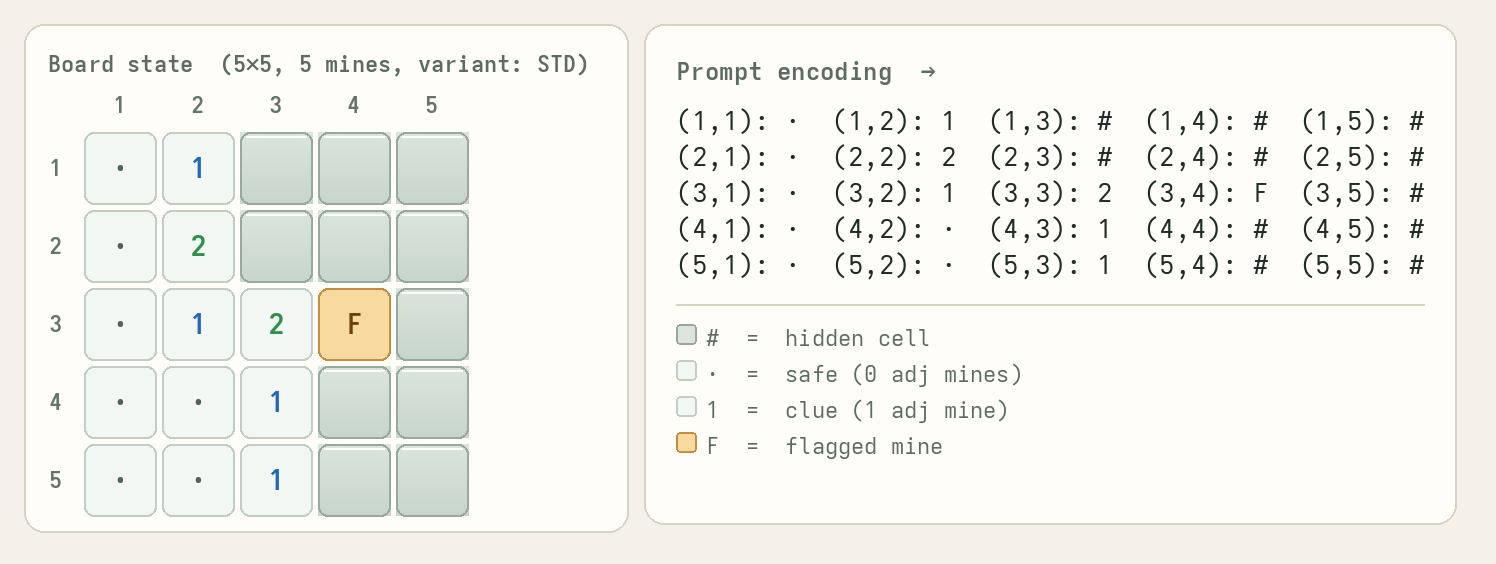
\includegraphics[width=1\linewidth]{board_example.png}
    \caption{An Example Board and the Text Representation In a Prompt}
    \label{fig:placeholder}
\end{figure}

I ran 5-7 sessions per variant (total 64) drawn from the first available puzzles in the dataset. The experiment consumed 313,315 input tokens and 411,783 output tokens in total.


\section{Results}

\subsection{Win Rate by Variant}

\begin{table*}[t]
\centering
\small
\begin{tabular}{@{}lrrrrrr@{}}
\toprule
Variant & Sessions & Wins & Win Rate & REVEALs & Mine Hits & Hit Rate \\
\midrule
STD & 7 & 6 & \textbf{86\%} & 25  & 1 &  4.0\% \\
Dual   & 5 & 4 & \textbf{80\%} & 28  & 1 &  3.6\% \\
RowCol   & 6 & 4 & \textbf{67\%} & 36  & 2 &  5.6\% \\
Snake   & 6 & 4 & \textbf{67\%} & 28  & 2 &  7.1\% \\
Outside   & 5 & 3 & \textbf{60\%} & 12  & 2 & 16.7\% \\
Triple   & 5 & 3 & \textbf{60\%} & 15  & 2 & 13.3\% \\
Horizontal   & 5 & 2 & \textbf{40\%} & 15  & 3 & 20.0\% \\
Connected   & 5 & 1 & \textbf{20\%} & 23  & 4 & 17.4\% \\
Liar   & 5 & 0 &  \textbf{0\%} &  5  & 5 & 100\%  \\
Partition   & 5 & 0 &  \textbf{0\%} &  5  & 5 & 100\%  \\
Quad   & 5 & 0 &  \textbf{0\%} & 15  & 5 & 33.3\% \\
Cross (X)   & 5 & 0 &  \textbf{0\%} &  8  & 5 & 62.5\% \\
\bottomrule
\end{tabular}
\vspace{2pt}
\caption{Win rate and REVEAL mine-hit rate by variant. The deterministic solver achieves 100\% on all 600 puzzles.}
\label{tab:winrate}
\end{table*}
Table \ref{tab:winrate} shows win rates, session counts, and the rate at which an attempted reveal action hit a mine for each given variant. The model achieves an overall win rate of 42.2\% (27/64 sessions).

\subsection{Speed of Failure}
\begin{figure}[htp]
    \centering
    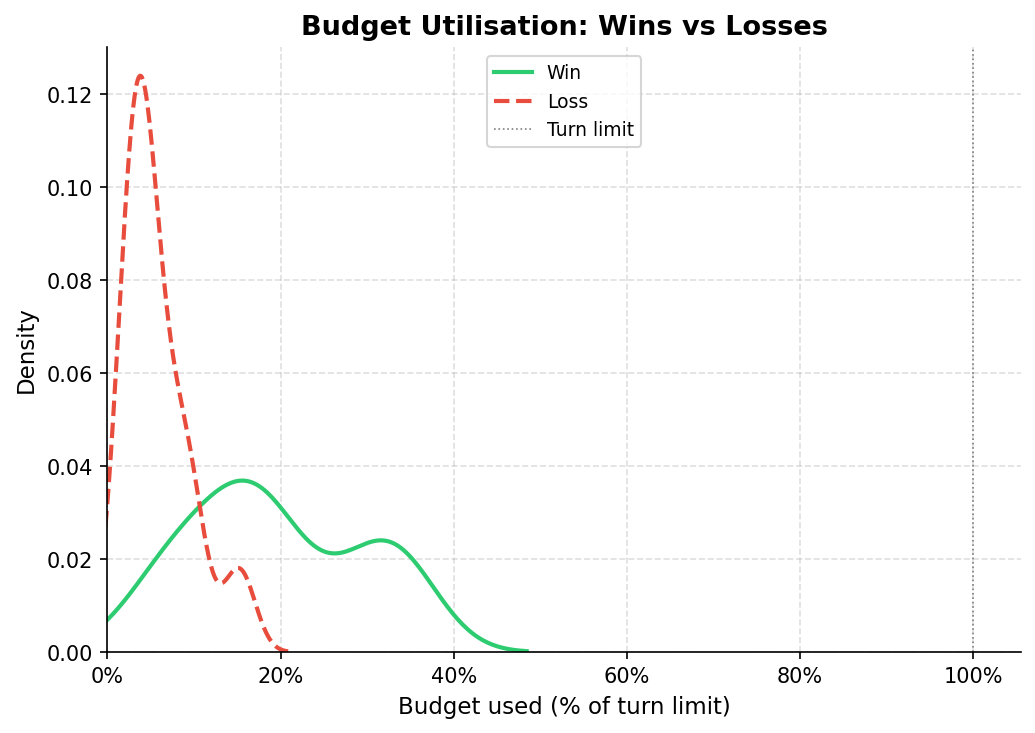
\includegraphics[width=1\linewidth]{budget_utilisation.png}
    \caption{The Density of Budget Usage}
    \label{fig:speed}
\end{figure}

The above figure \ref{fig:speed} depicts how much of the turn budget the model used for winning vs losing runs, relative to the turn limit that was determined by a factor of how long the deterministic solver took to complete the puzzle. Notably, this graph depicts that when losses occurred, they typically occurred in the first turn or two of play, indicating that most losses could likely be attributed to the model fundamentally failing to understand its objectives for a given variant.

\subsection{Action Mix}
\begin{figure}[htp]
    \centering
    
\includegraphics[width=1\linewidth]{action_mix.png}
    \caption{The Proportion of FLAG vs REVEAL Actions by Variant}
    \label{fig:actionproportion}
\end{figure}
Across all sessions, REVEAL accounts for the vast majority of moves, which aligns with expectations regarding the number of mines on the board. The zero-win variants show very low proportions of flagging, indicating that the model wasn't confident enough in mine identification and preferred to branch out for more information first. Notably, Snake achieves a high $67\%$ winrate with a very low FLAG rate of about $10\%$, which will be discussed more later.

\subsection{Qualitative Analysis: The Liar Variant}


The Liar variant produces the starkest failure mode and the most informative failure
trace. In Liar, each revealed clue is exactly $\pm 1$ away from the true adjacent mine
count (direction determined by cell parity). A cell with zero true adjacent mines
displays a $1$; a cell with one true adjacent mine displays a $0$ or a $2$.

A representative losing session shows the following reasoning from the model on turn 1:

\begin{quote}
\textit{``Cell (5,3) is hidden (\#) and is adjacent to both (5,2) and (5,4), which
are both `.' (zero mines). Therefore (5,3) must be safe to reveal.''}
\end{quote}

The model's logical inference is correct under standard Minesweeper semantics where a cell
adjacent only to zeros is safe. But in the Liar variant, displayed zeros are actually
$1$s (one true adjacent mine), so the inference is systematically wrong. The
model reveals cell (5,3), which contains a mine. A pattern mirroring this one occurs on the very first move
in every Liar session, with no variance in this small sample.

The session log shows the model explicitly referencing the Liar variant rule in the
system prompt but then reasoning from standard clue semantics anyway. The rule
description appears to be comprehended at the surface level (the model can reproduce it), but it
does not propagate into the underlying inference procedure.

\section{Discussion}
\subsection{Clue Semantics vs. Structural Constraints}
My initial hypothesis was that global structural constraints on the orientation of the mines would be more difficult for the model to maintain consistency with this rule as it made moves, but the experiments conducted provide evidence against that idea.

The data shows a pattern in the direct opposite direction. Global structural constraints (D, S, R, O, T) result in moderate to good performance overall, though displaying some variance with such a small sample, while variants that modify the clues themselves (L, P, X) result in total failure. The structural variants add information that restrict mine placement, but the model was still able to make significant progress by applying default minesweeper logic to a puzzle that happens to not require heavy consideration of the constraint. However, observing some of the reasoning given the model was still considering these variants in many cases, and simply wasn't able to effectively utilize them to succeed.

In contrast to this, the variants that modify the semantic understanding of what the numeric clues are strongly penalize ignoring the variant and only using standard logic, and this is clearly demonstrated in the results.

\subsection{Why Liar and Partition Are Worse Than Random}
One of the most interesting results from this testing is that the performance on variants Liar and Partition is a lot worse than random chance. On a $5\times5$ board with 5 mines, there is a $20\%$ chance of hitting a mine if all squares are hidden. This goes up with the initially given revealed squares, but is only ever $100\%$ when the game is in a completed state with every safe space revealed. This result may have been a result of the system prompt continuing to describe the game as `Minesweeper', despite not following traditional rules, which led to incorrect assumptions that took precedent over the consideration of the variant. However, it strengthens the argument that LLMs perform well on tasks that involve incorporating additional information, but don't yet have the cognitive flexibility to fully recalibrate themselves away from a well learned pattern\cite{xu2024puzzlesurvey}.

\subsection{What the Model Got Right}
The variants that the model succeeded best with were those that changed the puzzle the least. Variants like Dual or Snake were examples of this, variants that enforced a structure on the mines but ultimately still allowing the model to succeed using mostly standard Minesweeper logic. Though some of the reasoning responses of the model do cite the variant (talking about things like the location of the snake of mines), the majority of successful turns taken during these puzzles appeared to be mostly related to standard logic.

One of the most interesting plots to come out of these experiments is Figure 3, which depicts the proportion of REVEAL actions in comparison to FLAG actions. In particular, I want to note the extremely low proportion of FLAG actions taken for the Snake variant, despite the very low hit rate as shown in Table 3. This result indicates that the model successfully identified that the goal of the puzzle is not to flag mines, but to reveal every safe space, and was capable of tracking the puzzle state well enough to not require mine flags to reach a solution. As a human Minesweeper player, this pattern fascinates me, because often while playing the game myself or watching others play the game, it is extremely difficult to succeed without an indication of previously completed logical deductions.

\subsection{Implications for Design}
Though this paper represents a toy task on a weak model without a massive sample size, the results do seem to have general implications for reasoning benchmarks. These variants are all applied in the same general pipeline, but the evaluations that modified semantic meaning seemed to test a different enough capability that this isn't the best way to test capabilities like this, and that further customization is needed.
Reassigning meaning to familiar symbols is difficult to do in the prompt space, especially while referencing tasks the model is familiar with, 


\section{Limitations}
The biggest limiting factor here was the cost of querying frontier language models. Using Anthropic's Haiku 4.5, the average cost to test a single puzzle from beginning to end was about $\$0.03$, but this increased substantially if the model did well in the puzzle and continued taking turns. There are a few main things that could be scaled with a higher budget that would improve both the rigor of the experiments, and potentially the quality of the results.

The first obvious one is the number of trials done. This paper attempted to cast a wide net with the number of variants examined and essentially tried to establish that this is an interesting way to view this problem, but running a statistically significant quantity of trials across this many types of puzzles wasn't feasible.

The other main issue was the cost of deeper reasoning processes for models. As discussed above, the allotted budget was a maximum of 2000 tokens per turn, but these tokens were output tokens, and cost a significant amount. Combined with the fact that some puzzles could take up to 20 turns, this is an extremely expensive number to scale. However, with more time and tokens to process the state of the puzzle, it is reasonable to expect that the models would be capable of doing even more complex reasoning.

Finally, the models used are a reflection of this limitation. The experiments were run on Haiku 4.5, which offers an impressive level of intelligence, but isn't necessarily as useful or generalizable as the result from the models on the edge of the frontier could be. For a stronger model, it is both more expensive to run the prompts necessary to complete a single turn, and the number of turns expected is higher, assuming the model performs better.

\section{Conclusion}

In this paper, I performed an evaluation of \texttt{claude-haiku-4-5} on twelve variants of Minesweeper puzzles, finding that the model achieves strong performance ($60\%-86\%$ winrate) on variants that preserve standard semantic meanings of clues, and zero wins on variants that alter what the displayed numbers mean. Losses are often abrupt, indicating a fundamental inability to interpret what the board state is and how to progress safely, rather than an accumulation of too much information to handle.

The clearest takeaway is a distinction between two types of rule adaptation:
\begin{itemize}[topsep=2pt,itemsep=2pt]
  \item \textbf{Additive constraints} (extra conditions on mine placement): the model
        partially incorporates these or benefits from their side effects on puzzle
        structure, achieving non-trivial win rates.
  \item \textbf{Semantic substitutions} (different meaning for the same displayed
        symbols): the model fails completely, performing worse than a random agent in
        some cases because its confident-but-misdirected reasoning steers it directly
        into mines.
\end{itemize}

This distinction may generalize beyond Minesweeper, implying that tasks that ask an LLM to fully reinterpret something it has come to understand well may be less successful than tasks that add new information to familiar tasks \cite{xu2024puzzlesurvey}, and it is useful to build off of known tasks carefully.

Future work should primarily focus on a few key areas for exploration. The first of those is to utilize a stronger model, like Anthropic's Sonnet or Opus, to see if they fall into the same trap of not being able to effectively internalize the rules that change clue semantics. In addition, it would be interesting to see how model performance changes based on grid size. Do the emergent reasoning capabilities that allow success on a standard puzzle hold for a $10\times10$ board? A $100\times100$ board? Additionally, the manner in which the present board is communicated to the model is a possible variable to be examined. If the model can still make the connection of an implicit coordinate structure based purely on a list of characters and row numbers separated by commas, that indicate another skill that is interesting to measure. Finally, additional work into the system prompt may alter the results described here. Things like having the model recite the variant rule back during each turn might improve results.

% trigger a \newpage just before the given reference
% number - used to balance the columns on the last page
% adjust value as needed - may need to be readjusted if
% the document is modified later
%\IEEEtriggeratref{8}
% The "triggered" command can be changed if desired:
%\IEEEtriggercmd{\enlargethispage{-5in}}

% references section

% can use a bibliography generated by BibTeX as a .bbl file
% BibTeX documentation can be easily obtained at:
% http://mirror.ctan.org/biblio/bibtex/contrib/doc/
% The IEEEtran BibTeX style support page is at:
% http://www.michaelshell.org/tex/ieeetran/bibtex/
\bibliographystyle{IEEEtran}
\bibliography{references}
% argument is your BibTeX string definitions and bibliography database(s)
%\bibliography{IEEEabrv,../bib/paper}
%
% <OR> manually copy in the resultant .bbl file
% set second argument of \begin to the number of references
% (used to reserve space for the reference number labels box)
% \begin{thebibliography}{1}

% % \bibitem{IEEEhowto:kopka}
% % H.~Kopka and P.~W. Daly, \emph{A Guide to \LaTeX}, 3rd~ed.\hskip 1em plus
% %   0.5em minus 0.4em\relax Harlow, England: Addison-Wesley, 1999.

% \end{thebibliography}
\pagebreak



% that's all folks
\end{document}


